\begin{figure}[hpt!]
\centering

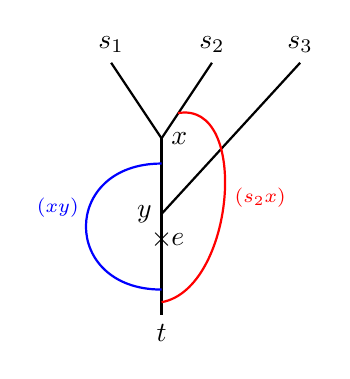
\begin{tikzpicture}[scale=1.6]
\begin{scope}
\coordinate (s2) at (0.4,2);
\coordinate (s1) at (-0.4,2);
\coordinate (s3) at (1.1,2);
\coordinate (x) at (0,1.4);
\coordinate (y) at (0,0.8);
\coordinate (t) at (0,0);
\coordinate (ts) at (0.15,0.4);
\coordinate (b1) at (0,.2);


\coordinate (a1) at (0,1.2);
\coordinate (a2) at (0.13,1.6);
\coordinate (v) at (0,.6);

\coordinate (c) at (-0.7,0.66);
\coordinate (b2) at (0,0.1);

\draw[thick](s1)--(x);
\draw[thick](s3)--(y);
\draw[thick](s2)--(x);
\draw[thick](x)--(t);
\node[above] at (s2){$s_2$};
\node[above] at (s1){$s_1$};
\node[above] at (s3){$s_3$};
\node[below] at (t){$t$};


\node[left] at (y){$y$};
\node[right] at (x){$x$};


\draw[blue,thick] (a1) to[out=180,in=180,distance=.8cm]
node[pos=0.4,left]
{\scriptsize  $\TON(xy)$}  (b1);



\draw[red,thick] (a2) to[out=10,in=10]
node[pos=0.5,right]
{\scriptsize  $\TON(s_2x)$}  (b2);

\node at (v){$\times$};
\node[right] at (v){$e$};

\end{scope}

\end{tikzpicture}
\caption{The shortest path from $s_2$ to $t$ avoiding $e$ can be $\TON(xy)$ or $\TON(s_2x)$.}
\label{fig:heavylight}

\end{figure}
